\documentclass{beamer}

\usepackage{lmodern}
\usepackage[utf8]{inputenc}
\usepackage[T1]{fontenc}
\usepackage[french]{babel}
\usepackage{url}
\usepackage{listings}
\usepackage{graphicx}
\usepackage{pifont}
\usepackage{changepage}
\usepackage{xcolor}

\graphicspath{ {../doc/img/} }

\newcommand{\cmark}{\ding{51}}
\newcommand{\xmark}{\ding{55}}

\definecolor{tomato}{rgb}{1.0, 0.39, 0.28}
\definecolor{gold}{rgb}{1.0, 0.84, 0.0}
\definecolor{mediumseagreen}{rgb}{0.24, 0.7, 0.44}

\usetheme{Madrid}
\usecolortheme{default}

\title[Analyse de données d'eye-tracking]{Analyse de données d'eye-tracking}
\subtitle{Travail d'Etude et de Recherche}
\author[STAVRIDIS Adonis]{STAVRIDIS Adonis}
\institute[Unistra, iCube]{
  Université de Strasbourg \and iCube \and 
  Antonio Capobianco, Flavien Lécuyer
}
\date[TER]{25 Mai 2021}

\begin{document}

\setbeamertemplate{caption}{\raggedright\insertcaption\par}

%-------------------------------------------------------------------------------
\frame{\titlepage}
%-------------------------------------------------------------------------------
\begin{frame}{Introduction}
  \begin{block}{Eye-tracking / Oculométrie}
    processus d'enregistrement du regard
  \end{block}
  \pause
  \begin{figure}
    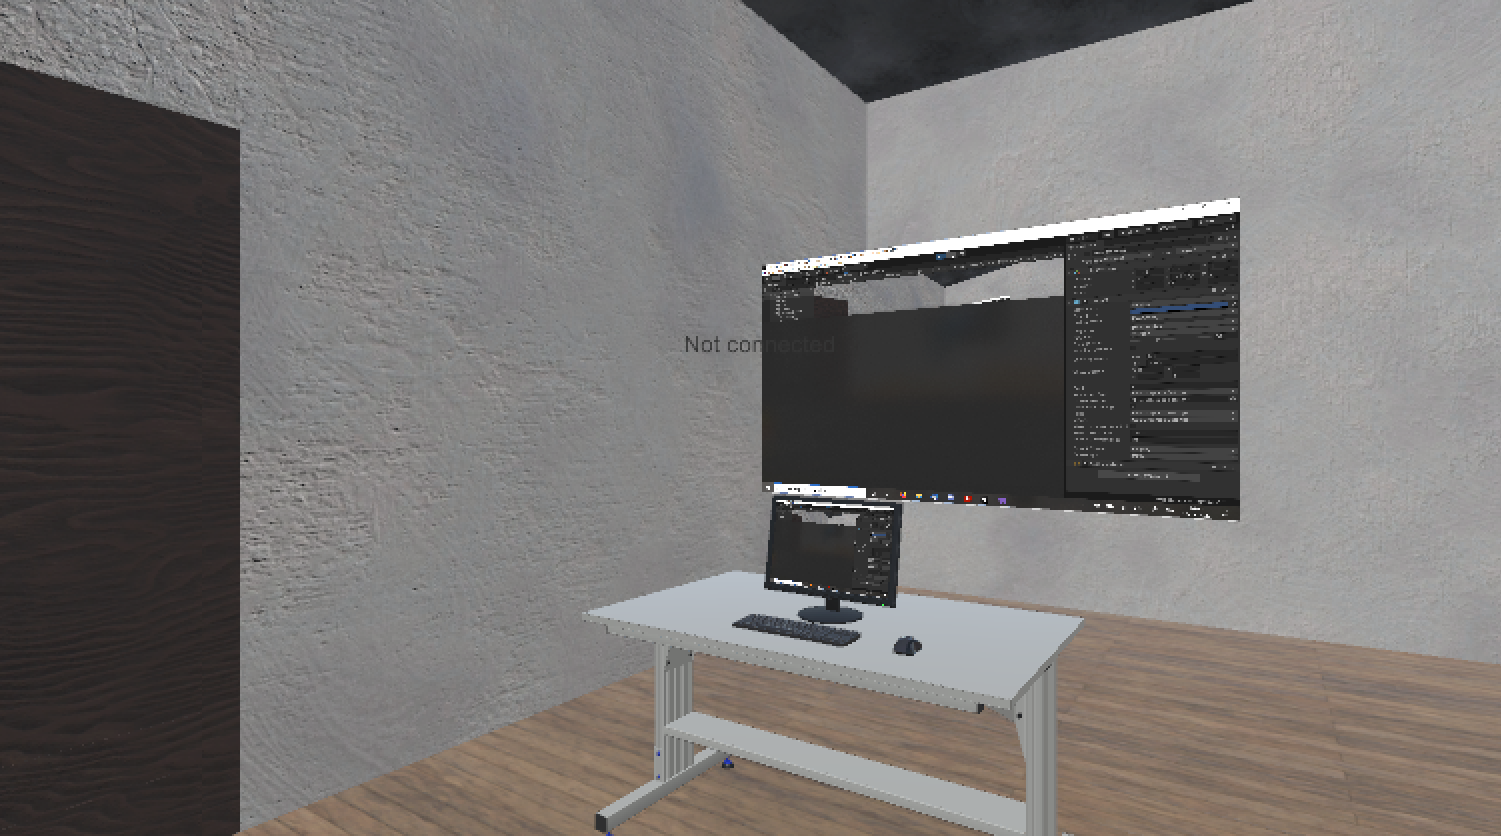
\includegraphics[height=0.35\textwidth]{environnement.png}
    \caption{Environnement de travail virtuel}
  \end{figure}
\end{frame}
%-------------------------------------------------------------------------------
\begin{frame}
  \frametitle{Sommaire}
  \tableofcontents
\end{frame}
%-------------------------------------------------------------------------------
\section{Capteurs}
%-------------------------------------------------------------------------------
\begin{frame}{Capteurs}
  \begin{columns}
    \column{0.5\textwidth}
    \begin{figure}
      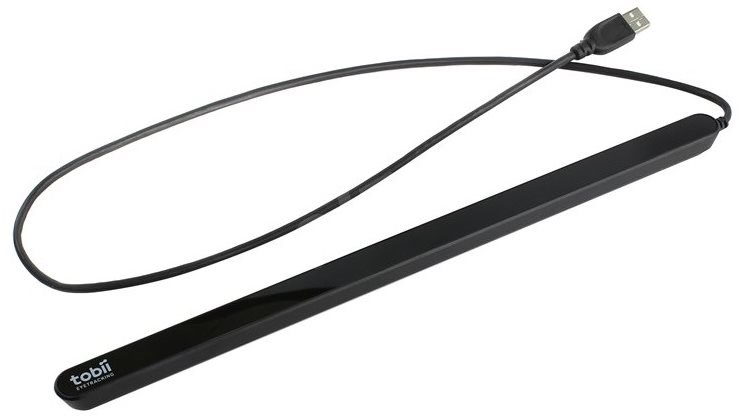
\includegraphics[height=0.35\textwidth]{tobii.jpeg}
      \caption{Capteur d'écran Tobii}
    \end{figure}
    \column{0.5\textwidth}
    \begin{figure}
      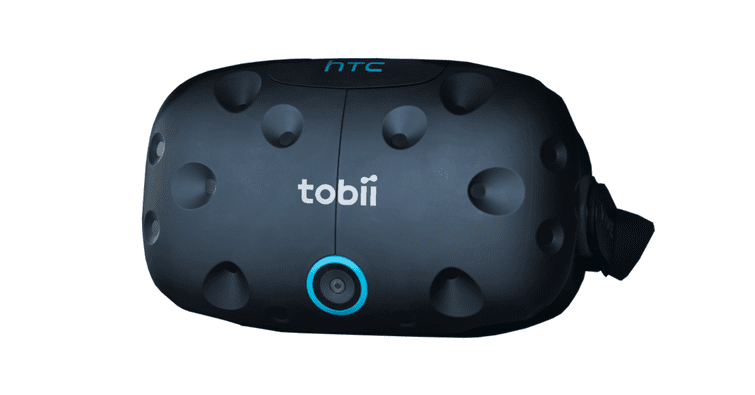
\includegraphics[height=0.35\textwidth]{htcvive.png}
      \caption{Casque de réalité virtuelle avec capteurs intégrés}
    \end{figure}
  \end{columns}
\end{frame}
%-------------------------------------------------------------------------------
\section{Analyse des données}
%-------------------------------------------------------------------------------
\begin{frame}[fragile]{Analyse des données}
  \begin{lstlisting}
    <temps> : <positionX>, <positionY>
    0.00 : 50, 50
    0.25 : 43, 64
    0.50 : 38, 75
    0.75 : 41, 66
    ...
  \end{lstlisting}
\end{frame}
%-------------------------------------------------------------------------------
\begin{frame}{Analyse des données}
  \begin{figure}
    \includegraphics<1>[height=0.5\textwidth]{raw.png}
    \includegraphics<2>[height=0.5\textwidth]{heatmap.png}
    \caption{
      \only<1>{Positions des fixations}
      \only<2>{Carte de chaleur}
    }
  \end{figure}
\end{frame}
%-------------------------------------------------------------------------------
\section{Logiciels}
%-------------------------------------------------------------------------------
\begin{frame}{Logiciels}
  \begin{table}[htpb]
    \begin{center}
      \begin{tabular}{|c||c|c|c|}
        \hline
        Logiciels       & Flexibilité                               & Analyse                                   & Documentation                             \\
        \hline
        GazePointer     & \textcolor{red}{\xmark}                   & \textcolor{orange}{\cmark}                & \textcolor{orange}{\cmark}                \\
        Ogama           & \textcolor{red}{\xmark}                   & \textcolor{mediumseagreen}{\cmark \cmark} & \textcolor{orange}{\cmark}                \\
        \textbf{PyGaze} & \textcolor{mediumseagreen}{\cmark \cmark} & \textcolor{mediumseagreen}{\cmark \cmark} & \textcolor{mediumseagreen}{\cmark \cmark} \\
        GazeParser      & \textcolor{orange}{\cmark}                & \textcolor{mediumseagreen}{\cmark \cmark} & \textcolor{orange}{\cmark}                \\
        \hline
      \end{tabular}
      \caption{Comparaison des logiciels}
    \end{center}
  \end{table}
\end{frame}
%-------------------------------------------------------------------------------
\section{Implémentation}
%-------------------------------------------------------------------------------
\begin{frame}{Implémentation}
  \begin{itemize}
    \item Plusieurs formats de données
    \item Données volumineuses
  \end{itemize}

  \begin{table}[htpb]
    \begin{adjustwidth}{0.05\textwidth}{0cm}
      \begin{tabular}{|c||c|}
        \hline
        Temps  & Image  \\
        \hline
        0.0    & image1 \\
        7.3    & image2 \\
        \vdots & \vdots \\
        \hline
      \end{tabular}
      \newline
      \begin{tabular}{|c||c|c|c|c|c|}
        \hline
        Temps  & Fixs/X & Fixs/Y & Distance & Pup/Gauche & Pup/Droite \\
        \hline
        0.0    & 43.2   & 57.8   & 0.5      & 2.8        & 2.8        \\
        4.7    & 34.4   & 49.6   & 0.4      & 2.8        & 2.8        \\
        8.1    & 30.7   & 52.1   & 0.4      & 2.8        & 2.8        \\
        \vdots & \vdots & \vdots & \vdots   & \vdots     & \vdots     \\
        \hline
      \end{tabular}
    \end{adjustwidth}
    \caption{\centering Format des données d'un fichier csv template
      (temps en microsecondes, fixations en pourcentage, distance en mètre,
      diamètre de la pupille en millimètre)}
  \end{table}
\end{frame}
%-------------------------------------------------------------------------------
\section{Résultats}
%-------------------------------------------------------------------------------
\begin{frame}{Résultats}
  \begin{figure}
    \includegraphics<1>[height=0.5\textwidth]{tea-raw-9.png}
    \includegraphics<2>[height=0.5\textwidth]{tea-heatmap-9.png}
    \caption{
      \only<1>{Points de fixations}
      \only<2>{Carte de chaleur}
    }
  \end{figure}
\end{frame}
%-------------------------------------------------------------------------------
\begin{frame}{Résultats}
  \begin{figure}
    \includegraphics<1>[height=0.5\textwidth]{vr-raw-0.png}
    \includegraphics<2>[height=0.5\textwidth]{vr-heatmap-0.png}
    \caption{
      \only<1>{Points de fixations}
      \only<2>{Carte de chaleur}
    }
  \end{figure}
\end{frame}
%-------------------------------------------------------------------------------
\begin{frame}{Conclusion}
  Travail réalisé
  \begin{itemize}
    \item Traitement de deux formats de données spécifiques
    \item Création de cartes de points de fixation et de chaleur
  \end{itemize}

  Limites
  \begin{itemize}
    \item Fonctionnalités
  \end{itemize}

  Pour aller plus loin
  \begin{itemize}
    \item Plus des fonctionnalités
    \item Application à la 3D pour la réalité virtuelle
  \end{itemize}
\end{frame}
%-------------------------------------------------------------------------------

\end{document}
